
\section{3. Puente de medici\'on de capacitores}
El objetivo de esta secci\'on es realizar el an\'alisis y dise\~no de un circuito puente denominado C Serie, con el fin de poder medir diferentes tipos de capacitores de prueba, tanto su par\'ametro de capacidad como factor de p\'erdidas del mismo.

\begin{figure}[H]
    \centering
    \includegraphics[scale=0.7]{Recursos/cserie.png}
    \caption{Puente C Serie}
    \label{fig:puente_c_serie}
\end{figure}

\subsection{An\'alisis te\'orico}
Se propone establecer un valor fijo para el capacitor patr\'on $C_1$ y la resistencia $R_4$, as\'i se utilizan $R_3$ y $R_1$ como variables de ajuste para llevar al puente a la condici\'on de equilibrio, para lo cual se definir\'a en cada caso un valor m\'inimo y m\'aximo seg\'un los rangos de operaci\'on del puente de medici\'on. 
Vale mencionar que para implementar el rango de variaci\'on de las variables de ajuste, se har\'a uso de una resistencia en serie junto con presets o trimmers de diferentes valores para garantizar tanto un ajuste grueso como fino del puente.

\subsubsection{Condiciones de dise\~no}
Se desea dise\~nar un puente de medici\'on C Serie que opere a una frecuencia de $f = 20kHz$. Debe ser capaz de medir capacitores que se encuentren dentro del rango $10nF < C < 100nF$ y $0.02 < D < 0.12$.

\subsubsection{Ecuaciones del puente}
\begin{equation}
\begin{array}{lllll}
    \frac{V_d}{V_g} = \frac{Z_3\cdot Z_x - Z_4 \cdot Z_1}{Z_1 \cdot Z_x + Z_1 \cdot Z_4 + Z_3\cdot Z_x + Z_3 \cdot Z_4}\\
    Z_1 = \frac{1}{s\cdot C_1} + R_1\\
    Z_x = \frac{1}{s\cdot C_x} + R_x\\
    Z_3 = R_3\\
    Z_4 = R_4\\
\label{eq:Ec_puente}
\end{array}
\end{equation}

\subsubsection{Sensibilidades del puente}
El proceso de medici\'on de un puente requiere alcanzar la condici\'on de equilibrio a trav\'es del ajuste de sus diversas variables, para lo cual es de inter\'es conocer con qu\'e sensibilidad var\'ia la condici\'on respecto de los cambios en tales variables. Para este an\'alisis se emplea la definici\'on de sensibilidad absoluta, asumiendo cambios o variaciones no muy grande se hace un c\'alculo en diferencias de las variables.

\paragraph{Sensibilidad respecto de la variable $Z_3$}

\begin{equation}
    V_d + \Delta V_d=\frac{(Z_3+ \Delta Z_3)\cdot Z_x - Z_4 \cdot Z_1}{Z_1 \cdot Z_x + Z_1 \cdot Z_4 + (Z_3+ \Delta Z_3)\cdot Z_x +(Z_3+ \Delta Z_3) \cdot Z_4} \cdot V_g
    \label{eq:Sensibilidad_Z3_1}
\end{equation}

\begin{equation}
     Z_3 \gg \Delta Z_3 \Rightarrow
    \Delta V_d = \frac{\frac{\Delta Z_3}{Z_3}}{\left(\frac{Z_1}{Z_3}+ 1\right)\left(\frac{Z_4}{Z_x} + 1\right)} \cdot V_g
\end{equation}

Se define, asumiendo que se cumple la condici\'on de puente balanceado, $A=\frac{Z_1}{Z_3}=\frac{Z_x}{Z_4}$.

\begin{equation}
\Delta V_d = \frac{A}{(A+1)^2} \cdot \frac{\Delta Z_3}{Z_3} \cdot V_g = \frac{A}{(A+1)^2} \cdot \frac{\Delta R_3}{R_3} \cdot V_g 
\label{eq:sens_z3_cabezapuente}
\end{equation}

\paragraph{Sensibilidad respecto de la variable $Z_1$}

\begin{equation}
    \Delta V_d = - \frac{\frac{\Delta Z_1}{Z_1}}{\left(\frac{Z_3}{Z_1}+ 1\right)\left(\frac{Z_x}{Z_4} + 1\right)} \cdot V_g
\end{equation}

 \begin{equation}
    \left| \frac{\Delta Z_1}{Z_1} \right| = \frac{\Delta R_1}{|Z_1|} = \frac{\frac{\Delta R_1}{R_1}}{\sqrt{1 + \left(\frac{1}{\omega \cdot C_1 \cdot R_1 }\right)^2}}
\end{equation}

\begin{equation}
    \frac{1}{\omega \cdot C_1 \cdot R_1 }\gg 1 \Rightarrow
    \left| \frac{\Delta Z_1}{Z_1} \right| = \frac{\Delta R_1}{R_1}\cdot\omega \cdot C_1 \cdot R_1 
\end{equation}

\begin{equation}
   \Delta V_d = - \frac{\frac{\Delta R_1}{R_1}\cdot\omega \cdot C_1 \cdot R_1 }{\left(\frac{Z_3}{Z_1}+ 1\right)\left(\frac{Z_x}{Z_4} + 1\right)} \cdot V_g
\end{equation}

\begin{equation}
   \Delta V_d = \frac{A}{(A+1)^2}\cdot \frac{\Delta Z_1}{Z_1}\cdot\omega \cdot C_1 \cdot R_1 \cdot V_g
\end{equation}

\subsubsection{Dimensionamiento del puente}
Se obtienen de la condici\'on de puente balanceado, las ecuaciones que se muestran en \ref{eq:D_C_R_x}. A partir de estas, y de las condiciones sobre los m\'aximos valores medibles de capacidad y factor de p\'erdidas que se observan en la Tabla \ref{tab:condiciones_de_diseno}, se obtienen valores l\'imite para los presets a utilizar al realizar la medici\'on.
\begin{equation}
    \centering
        \begin{array}{ccc}
            C_x = \frac{C_1\cdot R_3}{R_4}\\
            R_x = \frac{R_1 \cdot R_4}{R_3}\\
            D_x = \omega\cdot C_1 \cdot R_1
            
        \end{array} 
    \label{eq:D_C_R_x}
\end{equation}
\begin{table}[H]
\centering
\resizebox{0.4\textwidth}{!}{%
\begin{tabular}{ccl}
\hline
Par\'ametros & M\'inimo & M\'aximo \\ \hline
$C_x$ & 10nF & 100nF \\
$D_x $& 0.02 & 0.12 \\
f & \multicolumn{2}{c}{20KHz} \\ \hline
\end{tabular}%
}
\caption{Condiciones de dise\~no del puente}
\label{tab:condiciones_de_diseno}
\end{table}

Se fijan valores para $C_1$ y $R_4$ de $1nF$ y $100\Omega$ respectivamente. A partir de estos valores se obtiene un rango posible para $R_3$ y $R_1$ que permiten lograr el equilibrio en cualquier caso donde se cumplan las condiciones impuestas. Se muestran en la Tabla \ref{table:Rangos_pot}, los resultados de dicho an\'alisis. 

\begin{table}[H]
\centering
\begin{tabular}{ccc}
\hline
Resistencias & M\'inimo & M\'aximo \\ \hline
$R_1$ & $159.15 \Omega$ & $954.9 \Omega$ \\
$R_3 $& $1 k\Omega$ & $10 k\Omega$ \\
\end{tabular}
\caption{Rango de valores }
\label{table:Rangos_pot}
\end{table}

Finalmente, se propone utilizar una resistencia $R_1$ compuesta por el conjunto serie de una resistencia de $R = 150 \Omega$ en serie con dos presets, uno de $1k\Omega$ y uno de $100\Omega$ de forma tal que la precisi\'on del cambio pueda ajustarse con mayor o menor paso. De igual forma en $R_3$ con una resistencia de $1k \Omega$ y dos presets de $10k\Omega$ y $1k \Omega$.

\begin{figure}[H]
    \centering
    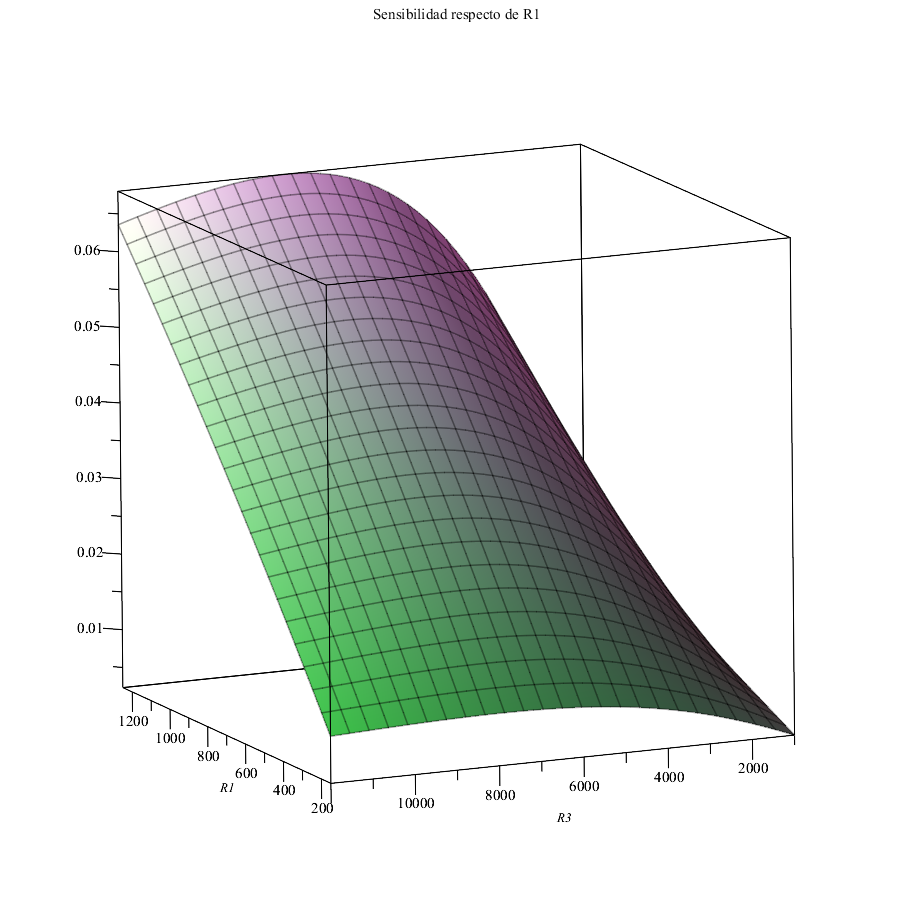
\includegraphics[scale=0.4]{Recursos/cserie_sensibilidad_r1.png}
    \caption{Sensibilidad respecto de R1}
    \label{fig:sensibilidad_r1}
\end{figure}

\begin{figure}[H]
    \centering
    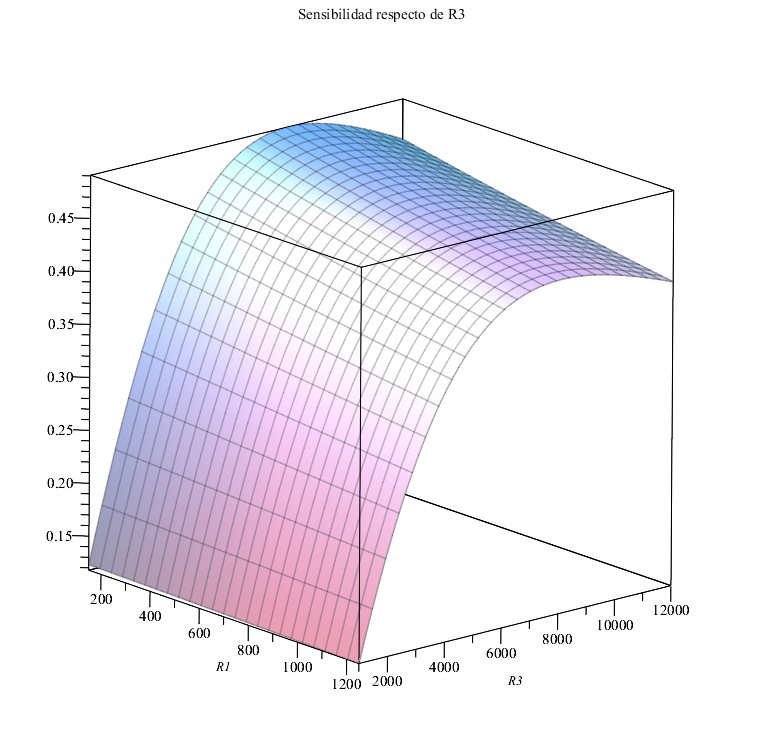
\includegraphics[scale=0.4]{Recursos/cserie_sensibilidad_r3.png}
    \caption{Sensibilidad respecto de R3}
    \label{fig:sensibilidad_r3}
\end{figure}

\begin{figure}[H]
    \centering
    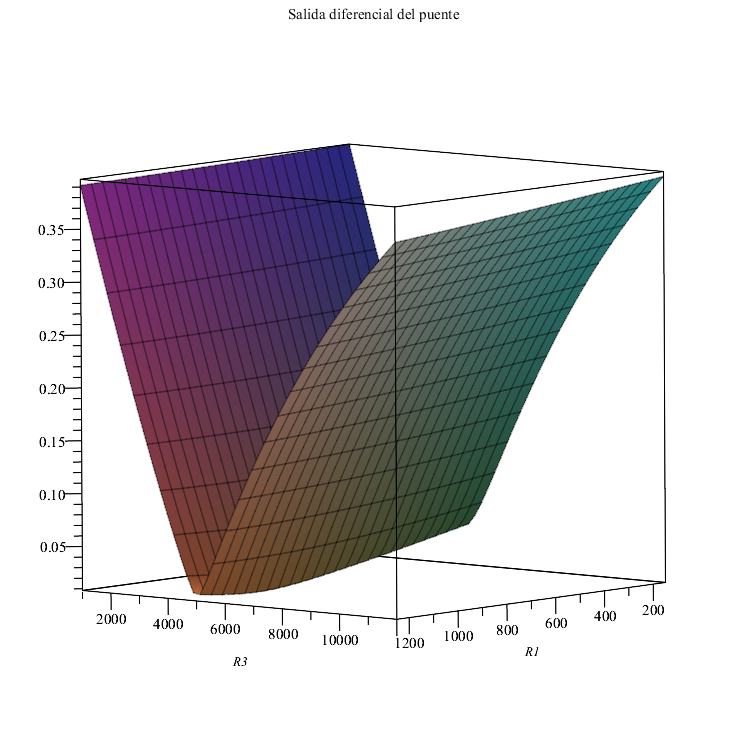
\includegraphics[scale=0.4]{Recursos/cserie_salida.png}
    \caption{Salida del puente variando R1 y R3}
    \label{fig:salida_puente_cserie}
\end{figure}



\subsection{Resultados}

\subsubsection{Componentes patr\'on}
Se emplea un analizador de impedancias para medir los componentes patr\'on utilizados en la implementaci\'on f\'isica del circuito puente. En ambos casos sea realiza la medici\'on con una frecuencia de  $f = 2kHz$, $f = 20kHz$ y $f = 200kHz$

\begin{table}[H]
    \centering
    \begin{tabular}{c c c c}
        $f [Hz]$ & $R [\Omega]$ & $C [F]$ & $D$ \\
        \hline \\
        $2kHz$ & $98.68\Omega$ & $955pF$ & $0.088$ \\
        $20kHz$ & $98.68\Omega$ & $938pF$ & $0.098$ \\
        $20kHz$ & $98.68\Omega$ & $926pF$ & $0.0145$ \\
        \hline
    \end{tabular}
    \caption{Componentes patr\'on del puente}
    \label{tab:mediciones_componentes_patron}
\end{table}

\subsubsection{Mediciones del puente}
Se utilizan diferentes capacitores arbitrarios como elementos de prueba del proceso de medici\'on empleando el puente dise\~nado. Se realizan las mediciones para las frecuencias de $f = 2kHz$, $f = 20kHz$ y $f = 200kHz$.

\begin{table}[H]
    \centering
    \begin{tabular}{c | c c c  c c c  c c c}
         Valor Nominal & \multicolumn{3}{c}{$f = 2kHz$} & \multicolumn{3}{c}{$f = 20kHz$} & \multicolumn{3}{c}{$f = 200kHz$} \\
         & $C$ & $D$ & $\phi$ & $C$ & $D$ & $\phi$ & $C$ & $D$ & $\phi$  \\
         \hline \\
         $10nF$ & $12.5nF$ &0.016 &$-89.05^\circ$& $9.79nF$&0.16&$-80.76^\circ$ &$9.29nF$ &1.64 &$-31.37^\circ$ \\
         $47nF$ & $43.9nF$&0.016 & $-89.03^\circ$& $48.1nF$&0.087 &  $-85.01^\circ$& $45.5nF$& 0.173&$-80.16^\circ$  \\
         $100nF$ & $105nF$& 0.006& $-89.62^\circ$& $105nF$ &0.025 &$-88.51^\circ$ &$107nF$ & 0.256&$-75.64^\circ$  \\
         $220nF$ &$107nF$ &0.003 & $-89.77^\circ$&$105nF$ & 0.033& $-88.1^\circ$&$104nF$ & 0.173& $-80.16^\circ$ \\
         \hline
    \end{tabular}
    \caption{Mediciones del puente}
    \label{tab:mediciones_del_puente}
\end{table}

\subsubsection{Mediciones del analizador de impedancias}
Se utiliza el analizador de impedancia para medir los mismos componentes arbitrarios que fueron medidos con el puente para realizar una apreciaci\'on de las diferencias. Se realizan las mediciones para las frecuencias de $f = 2kHz$, $f = 20kHz$ y $f = 200kHz$.

\begin{table}[H]
    \centering
    \begin{tabular}{c | c c c  c c c  c c c}
         Valor Nominal & \multicolumn{3}{c}{$f = 2kHz$} & \multicolumn{3}{c}{$f = 20kHz$} & \multicolumn{3}{c}{$f = 200kHz$} \\
         & $C$ & $D$ & $\phi$ & $C$ & $D$ & $\phi$ & $C$ & $D$ & $\phi$  \\
         \hline \\
         $10nF$ & $9.57nF$ &0.856 &$-49.3^\circ$& $9.57nF$&0.097&$-84.4^\circ$ &$9.28nF$ &0.024 &$-88.58^\circ$ \\
         $47nF$ & $47.3nF$&0.174 & $-80.12^\circ$& $46.8nF$&0.027 &  $-88.45^\circ$& $46.1nF$& 0.023&$-88.63^\circ$  \\
         $100nF$ & $107nF$& 0.507& $-63.05^\circ$& $106nF$ &0.061 &$-86.42^\circ$ &$104nF$ & 0.025&$-88.59^\circ$  \\
         $220nF$ &$200nF$ &0.035 & $-87.92^\circ$&$180nF$ & 0.032& $-88.13^\circ$&$162nF$ & 0.029& $-88.34^\circ$ \\
         \hline
    \end{tabular}
    \caption{Mediciones del puente}
    \label{tab:mediciones_del_puente}
\end{table}

\subsection{Manual de usuario}

En la Fig. \ref{fig:circuito_puente_final} se muestra un esquema general del circuito puente dise\~nado en el cual se puede apreciar que las variables de ajuste son $R_1$ y $R_3$, utilizando tanto un preset de ajuste fino como grueso para ambos casos. Se dispone de una entrada y una salida al mismo, el objetivo del proceso de medici\'on es aplicar una se\~nal de entrada dada y medir la salida diferencial, variando el ajuste hasta alcanzar el equilibrio en el cual $V_d = 0$. Finalmente se usan el conjunto de ecuaciones \ref{eq:D_C_R_x} para obtener los resultados.

\begin{figure}[H]
    \centering
    \includegraphics[scale=0.4]{Recursos/puente.png}
    \caption{Esquema general del circuito dise\~nado}
    \label{fig:circuito_puente_final}
\end{figure}

En la Fig. \ref{fig:conexion_puente} se ilustra un esquema general de la conexi\'on del puente. Se debe utilizar un generador de funciones o se\~nales configurando el mismo con una senoidal de un valor de amplitud $V_G = 1 V_{PP}$ con la frecuencia a la cual se desea analizar el capacitor. Finalmente, se emplea un osciloscopio con dos canales para medir ambas salidas del dispositivo y utilizando la funcionalidad Math calcular la diferencia entre ellas, variando el ajuste hasta alcanzar el equilibrio del puente.

\begin{figure}[H]
    \centering
    \includegraphics[scale=0.5]{Recursos/manual_cserie.png}
    \caption{Esquema de conexi\'on}
    \label{fig:conexion_puente}
\end{figure}

\begin{table}[H]
    \centering
    \begin{tabular}{c | c c c}
        Magnitud & M\'in. & \'Optimo & M\'ax. \\
        \hline \\
        $f$ & $2kHz$ & $20kHz$ & $2kHz$ \\
        $V_G$ & $-$ & $1 V_{PP}$ & $-$ \\
        $R_1$ & $150 \Omega$ & $-$ & $1250 \Omega$ \\
        $R_3$ & $1k \Omega$ & $-$ & $12k \Omega$ \\
        $C_x$ & $10nF$ & $-$ & $100nF$ \\
        $D_x$ & $0.02$ & $-$ & $0.12$ \\
        \hline
    \end{tabular}
    \caption{Especificaciones}
    \label{tab:especificaciones}
\end{table}

\subsection{Precisi\'on del puente}
Se calcula, tomando las mediciones realizadas con el analizador de impedancias como valor real, el error relativo porcentual cometido en las mediciones. Esto permite tener una idea de la precis\'on del puente y en error cometido al medir.

Se calcula el error relativo como $E_{\%Rel} = \frac{Valor_{medido}-Valor_{real} }{Valor_{real}}\cdot 100$. Al hacer este calculo para todas las mediciones realizadas se obtiene la Tabla \ref{tab:TAB_ERROR}
\begin{table}[H]
    \centering
    \resizebox{0.4\textwidth}{!}{%
    \begin{tabular}{cccc}
     & Frecuencia (Hz) & $E_{Cx}$ & $E_{Dx}$ \\ \hline
     \multirow{3}{*}{10nF} & 2000 & 30.45\% & 98.07\% \\
     & 20000 & $2.31\%$ & $66.66\%$ \\
     & 200000 & $0.11\%$ & $6511.20\%$\\ \hline
    \multirow{3}{*}{47nF} & 2000 & $7.05\%$ & $90.31\%$ \\
     & 20000 & $2.77\%$ & $221.87\%$ \\
     & 200000 & $1.21\% $& $625.45\%$ \\ \hline
    \multirow{3}{*}{100nF} & 2000 & $1.51\%$ &$ 98.70\%$ \\
     & 20000 & $0.92\%$ & $58.04\% $\\
     & 200000 & $2.86\%$ & $924.01\%$ \\ \hline
    \multirow{3}{*}{220nF} & 2000 & $46.66\% $& $89.24\%$ \\
     & 20000 & $41.54\%$ & $2.55\%$ \\
     & 200000 & $35.99\%$ & $497.87\%$ \\ \hline
    \end{tabular}%
    }
    \caption{Error relativo de C y D medidos}
    \label{tab:TAB_ERROR}
    \end{table}

\subsection{Conclusi\'on}
Se puede observar que en cuanto a las mediciones de capacidad a 20KHz y cumpliendo con las condiciones de dise\~no originales, se ajustan muy bien a lo medido con el analizador de impedancias. Se observa un error m\'aximo de aproximadamente 3\%, que se encuentra en un rango correcto de error. 

Para 2KHz y 200KHz se observa un error mayor, sin embargo las mediciones siguen dentro de un rango bajo de error en la mayor\'ia de los casos. Se observa que el error m\'aximo cometido en estas condiciones es del 30.45\%, pero en promedio el error es del 7.2\%.

Para valores de capacidad por fuera de los rangos de dise\~no se observa un error mucho mayor, que se corresponde con lo esperado.

Por \'ultimo, se puede observar que las mediciones del factor de p\'erdidas incurre en un error muy grande. Se asume que esto se debe a un error en el dise\~no del puente sumado a un error de apreciaci\'on cometido al utilizar el osciloscopio para realizar las mediciones. 
